\section{Further questions}
% 1. Are some decisions in any of the models driven by the application’s amount?
% 2. Are there clear indications that the same employees are always involved in cases that are
% declined, approved or cancelled?
% 3. The process owner would like to see a comparison of the throughput times between the nonapproved
% applications, i.e. those cancelled or rejected by the applicant, and the approved
% applications. In particular, he/she is interested in the time between the moment in which an
% application is submitted and when it is approved, compared with the time between the
% application is submitted and it is rejected or cancelled. 

\subsection{Are some decisions in any of the models driven by the application's amount?}
For answering this question I had a look at the dotted charts of the whole data set and the three filtered ones, "Filtered App", "Pdoubledfiltered", "Filtered Work". As x-axis I chose "C:Activity classifier" and y-axis "T:AMOUNT\_REQ". Also I sorted the traces by the "AMOUNT\_REQ". Just for the layout I changed the color to "C: Activity classifier".

\begin{figure}[!htbp]
\centering
\begin{subfigure}{0.49\textwidth}
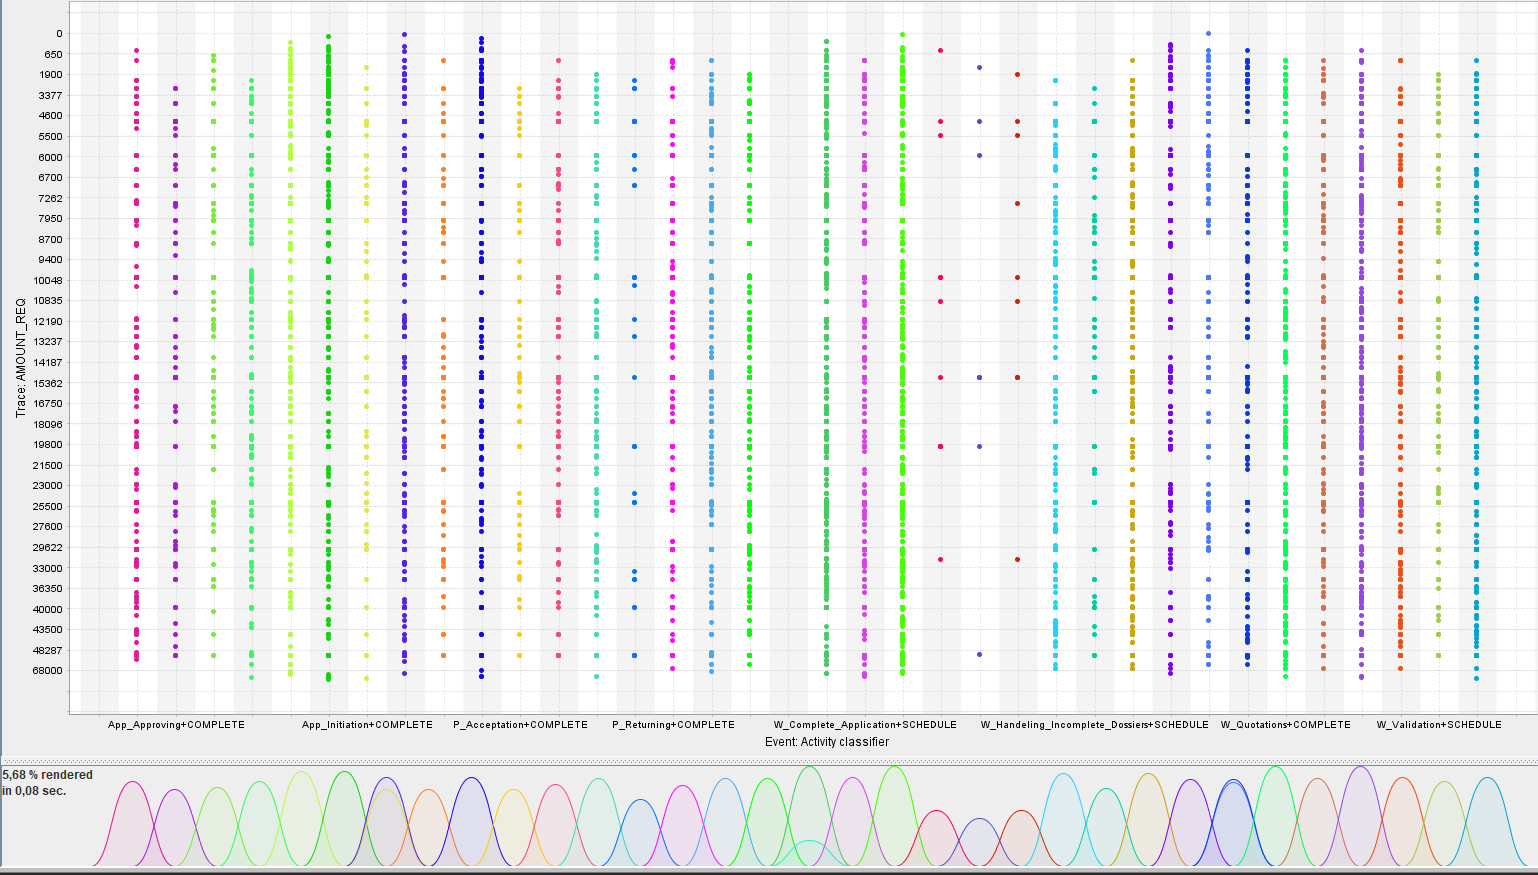
\includegraphics[width = 0.99\linewidth]{AmountRequ_All.PNG}
\caption{Whole data set}
\label{fig:AmounWhole}
\end{subfigure}
\begin{subfigure}{0.49\textwidth}
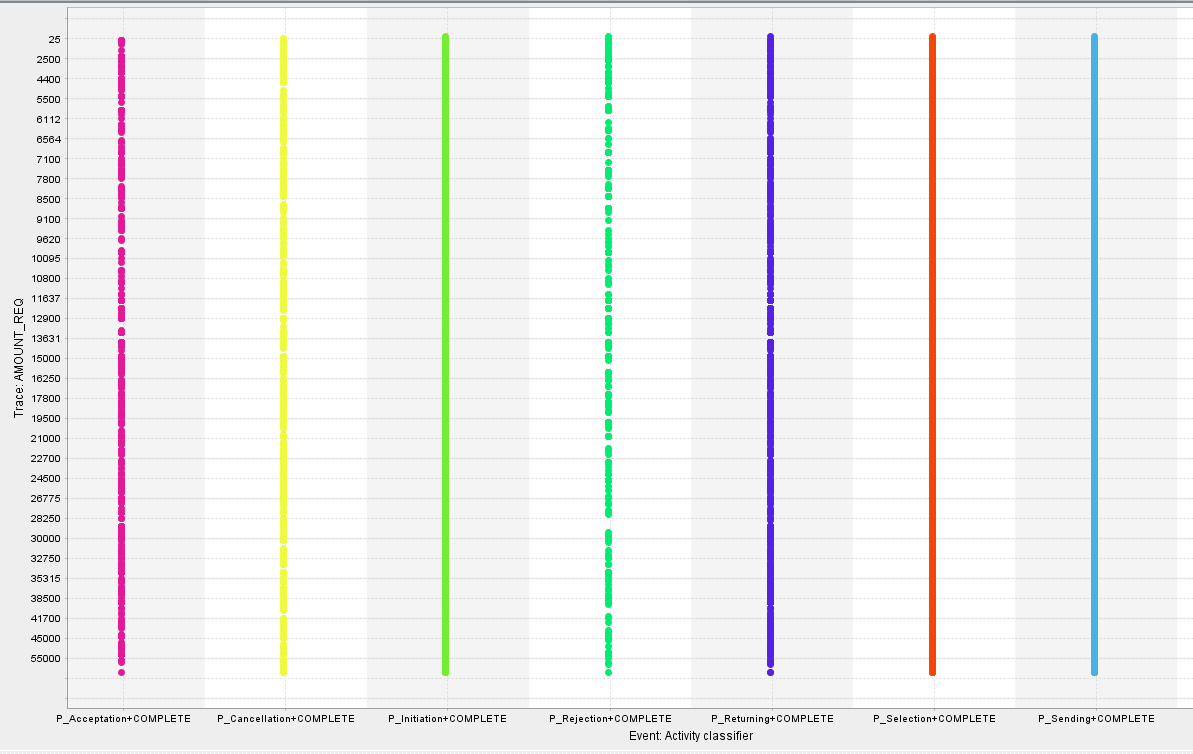
\includegraphics[width = 0.99\linewidth]{AmountRequ_P.PNG}
\caption{Proposal data set}
\label{fig:AmounP}
\end{subfigure}
\begin{subfigure}{0.49\textwidth}
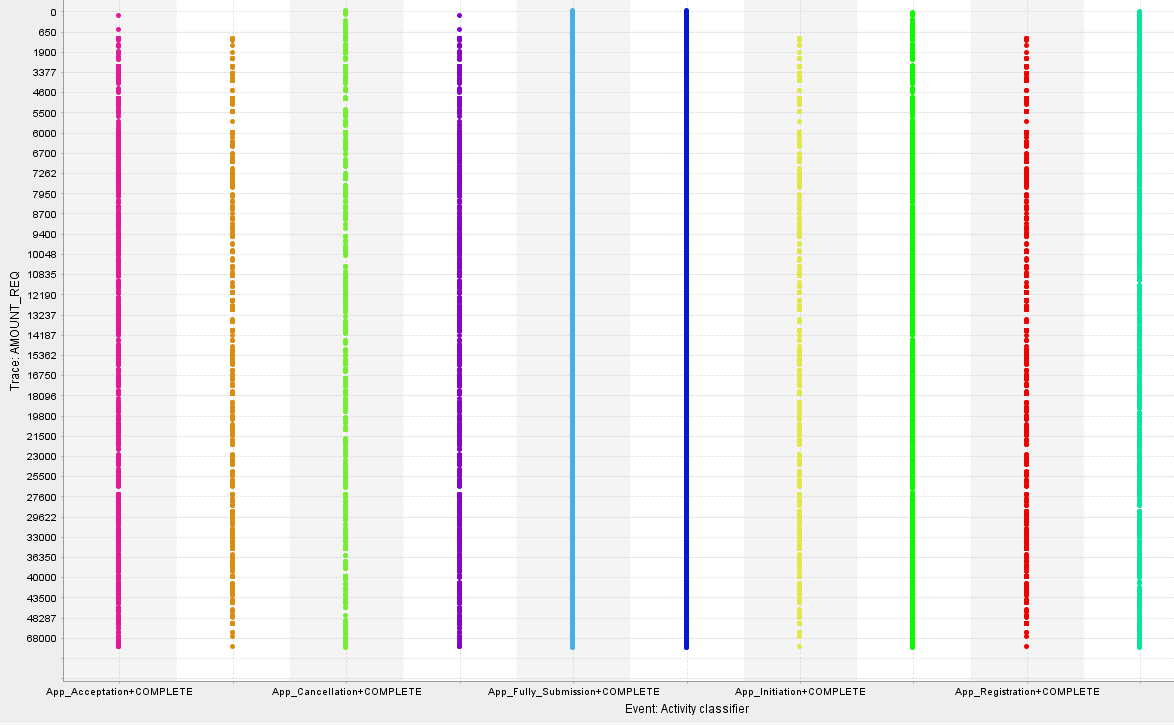
\includegraphics[width = 0.99\linewidth]{AmountRequ_App.PNG}
\caption{Application data set}
\label{fig:AmounApp}
\end{subfigure}
\begin{subfigure}{0.49\textwidth}
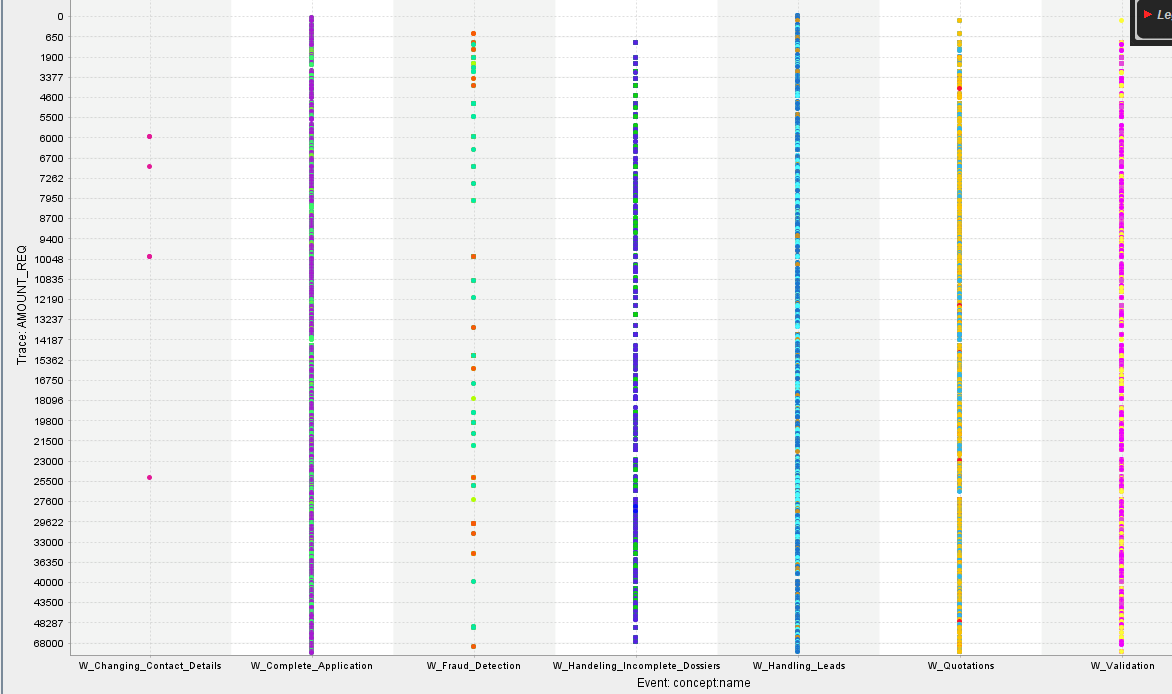
\includegraphics[width = 0.99\linewidth]{AmountRequ_Work.PNG}
\caption{Workflow data set}
\label{fig:AmounWhole}
\end{subfigure}
\caption{Dotted chart for the application's amount}
\label{fig:DotAmount}
\end{figure}

Figure \ref{fig:DotAmount} shows clearly, that there is \textbf{no correlation} between activity and requested amount. 

\subsection{Are there clear indications that the same employees are always involved in cases that are declined, approved or cancelled?}

For this question I concentrate on the application data set and filter it three time: "Filtered App with approv", where as end event just "APP\_Initation", "APP\_Registration" and "APP\_Approved" are possible as end event, based on the result of the 6th question before, where you can see, those three always happen together, "Filtered App with Rej", end event just "APP\_Rejected" and "Filtered App with Canc"

Those filtered data sets I used for the \textbf{Interactive Data aware Heuristic Miner}, where I chose resource in place of activity to create a model.

\subsubsection{Approved}

To see what are the main resources used I had a look at the c-net.
\begin{figure}[!htbp]
\centering
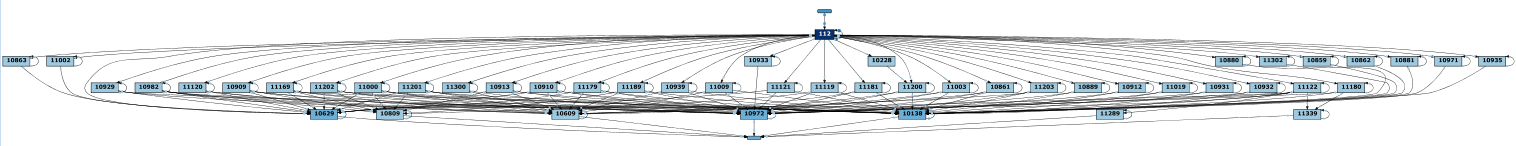
\includegraphics[width = 0.9\textwidth]{ApprovCnet.PNG}
\caption{Causal net of the approved application lifecyle without filtering}
\label{fig:CnetApprov}
\end{figure}

\begin{figure}[!htbp]
\centering
\begin{subfigure}{0.4\textwidth}
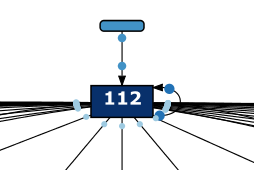
\includegraphics[width = 0.9\linewidth]{ApprovCnetBeginning.PNG}
\caption{Beginning of the traces}
\label{fig: CnetApprovBeg}
\end{subfigure}
\begin{subfigure}{0.4\textwidth}
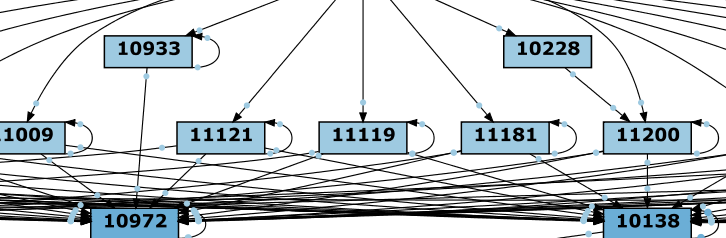
\includegraphics[width = 0.9\linewidth]{ApprovCnetMiddle.PNG}
\caption{Middle of the traces}
\label{fig: CnetApprovMid}
\end{subfigure}
\begin{subfigure}{0.9\textwidth}
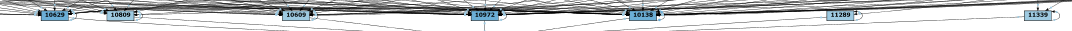
\includegraphics[width = 0.9\linewidth]{ApprovCnetEnd.PNG}
\caption{End of the traces}
\label{fig: CnetApprovEnd}
\end{subfigure}
\caption{Zoomed in the c-net}
\label{fig:CnetApprovZoome}
\end{figure}

There are three parts prominent, \ref{fig:CnetApprovZoome}:
\begin{enumerate}
	\item All traces start via \textbf{112}, \ref{fig: CnetApprovBeg}
	\item 2 resources, 10933 and 10228, just have two successors, \ref{fig: CnetApprovMid}
	\item 7 resources execute the last event, \ref{fig: CnetApprovEnd}
\end{enumerate}

\subsubsection{Rejected}

\begin{figure}[!htbp]
\centering
\begin{subfigure}{0.7\textwidth}
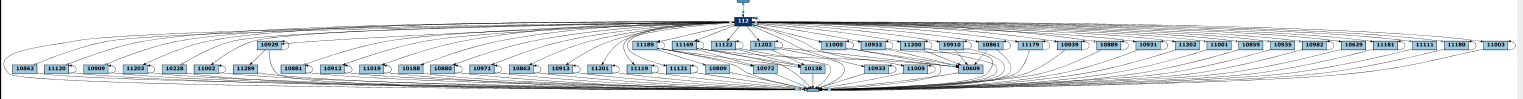
\includegraphics[width = 0.9\linewidth]{RejCNet.PNG}
\caption{Causal net of the reject application lifecyle without filtering}
\label{fig:CnetRej}
\end{subfigure}
\begin{subfigure}{0.2\textwidth}
\includegraphics[width = 0.9\textwidth]{RejCnetBeg.PNG}
\caption{Zoomed in the beginning of the c-net}
\label{fig:CnetRejZoome}
\end{subfigure}
\caption{Rejection resource c-net}
\label{fig:CnetRejto}
\end{figure}

Figure \ref{fig:CnetRej} shows the whole c-net and in \ref{fig:CnetRejZoome} it is more clear, that again \textbf{112} starts all traces.

\subsubsection{Cancellation} 

\begin{figure}[!htbp]
\centering
\begin{subfigure}{0.7\textwidth}
\includegraphics[width = 0.9\linewidth]{CancCNet.PNG}
\caption{Causal net of the cancellation application lifecyle without filtering}
\label{fig:CnetCanc}
\end{subfigure}
\begin{subfigure}{0.2\textwidth}
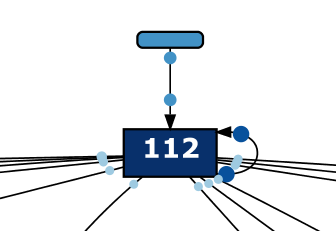
\includegraphics[width = 0.9\linewidth]{CancCnetBeg.PNG}
\caption{Zoomed in the beginning of the c-net}
\label{fig:CnetCancZoome}
\end{subfigure}
\caption{Cancellation resource c-net}
\label{fig:CnetCancto}
\end{figure}

Figure \ref{fig:CnetCanc} shows the whole c-net and in \ref{fig:CnetCancZoome} it is more clear, that again \textbf{112} starts all traces.

\subsubsection{Summary of those results}

So what gets pretty clear is that \textbf{112} decides over the next steps in the beginning. Having a look at the resources following it gets obvious, that different ressources work on the 3 sorts of traces. So it seems to depend on 112, which decision will be made.


\subsection{Comparsion of the throughput times}
%The process owner would like to see a comparison of the throughput times between the nonapproved applications, i.e. those cancelled or rejected by the applicant, and the approved
% applications. In particular, he/she is interested in the time between the moment in which an
% application is submitted and when it is approved, compared with the time between the
% application is submitted and it is rejected or cancelled. 

For this investigation I created a data set with the combination of rejected and cancelled traces, "Filtered App with rej and canc".

Then I looked the times up in the dotted chart like I did before.


\begin{figure}[!htbp]
\centering
\begin{tabular}{|c|c|c|c|}
\hline
& Minimum & Mean & Maximum \\ \cline{1-4}
Approved& $700910$ & $1.4393*10^9$ & $ 7419735534$      \\ \cline{1-4}
Rejected of cancelled  & $1855$ & $5.613*10^8$ & $7901736161$       \\ \cline{1-4}
\end{tabular}
\caption{Throughput times}
\label{tab:Throughtimes}
\end{figure}

In figure \ref{tab:Throughtimes} it can be clearly seen, that an approved traces takes 2.56 times so much time, than a rejected or cancelled trace. 
